\documentclass[11pt,letterpaper]{article}
\usepackage[margin=2cm]{geometry}
\usepackage{amsmath,amssymb,graphicx,xcolor,booktabs,tabularx,enumitem,titlesec,fancyhdr,array,longtable}
\usepackage{tikz}
\usetikzlibrary{arrows.meta,positioning,shapes.geometric,fit,calc,decorations.pathreplacing}
\usepackage[hidelinks]{hyperref}
\usepackage{helvet}\renewcommand{\familydefault}{\sfdefault}
\usepackage{caption}
\titleformat{\section}{\Large\bfseries\color{blue!50!black}}{\thesection}{0.6em}{}
\titleformat{\subsection}{\large\bfseries}{\thesubsection}{0.6em}{}
\titleformat{\subsubsection}{\normalsize\bfseries}{\thesubsubsection}{0.6em}{}
\setlength{\headheight}{14pt}
\setlist{itemsep=1pt,topsep=3pt}
\setlength{\emergencystretch}{3em}
\setlength{\parskip}{3pt}
\newcommand{\boxit}[4]{\par\medskip\noindent\fcolorbox{#1}{#2}{\begin{minipage}{0.955\linewidth}\textbf{#3}\par\smallskip #4\end{minipage}}\par\medskip}
\newcommand{\conceptbox}[2]{\boxit{blue!50!black}{blue!4}{#1}{#2}}
\newcommand{\connectbox}[1]{\boxit{green!40!black}{green!5}{Connect to your analysis}{#1}}
\newcommand{\pitfallbox}[1]{\boxit{red!60!black}{red!4}{Pitfalls}{#1}}
\newcommand{\checksbox}[1]{\boxit{orange!70!black}{orange!6}{Checks}{#1}}
\newcommand{\goal}[1]{\par\noindent\textbf{Goal.} #1\par}
\newcommand{\exbox}[2]{\boxit{gray!60!black}{gray!6}{Optional exercise #1}{#2}}
\pagestyle{fancy}\fancyhf{}\lhead{sPHENIX Self-Paced Course}\rhead{Module 6: Fun4All and Simulation}\cfoot{\thepage}
\begin{document}
\begin{center}
{\LARGE\bfseries sPHENIX Self-Paced Course --- Module 6:}\\[4pt]
{\Large\bfseries Fun4All framework, software stack and simulation}\\[8pt]
November 2026 \quad Prepared for P.\,D.\ Lewis (Ohio University)\\[2pt]
\small Self-contained study text based on the Summer-2026 sPHENIX School, public sPHENIX documents and standard textbook material
\end{center}

\tableofcontents
\newpage

\section*{How to use this module}
\addcontentsline{toc}{section}{How to use this module}
This module is self-contained. You do not need the school slides, the recordings or the papers to follow it.
Every concept is built up from first principles and then connected to the way sPHENIX actually does it.
The school talks listed below are the sources the text was distilled from; they are listed for reference only.

\subsection*{Learning objectives}
After this module you should be able to:
\begin{enumerate}[label=O\arabic*.]
\item Explain what the Fun4All server does in each phase of a job and why the framework is organised around a node tree.
\item Write, build, install and run a Fun4All macro with your own \texttt{SubsysReco} module, from an empty directory.
\item Navigate the node tree, find an object by name and class, and choose the right input and output managers.
\item Explain why sPHENIX classes are versioned behind virtual base classes (schema evolution) and what this means for your code.
\item Use the conditions database (CDB) through a global tag and a timestamp, and know what can go wrong.
\item Describe how Geant4 transports particles, what a G4Hit is, and how simulated hits become towers that the data reconstruction can read.
\item Configure event generators (PYTHIA8, HIJING via HepMC, single-particle guns) and explain sim-into-sim and sim-into-data embedding.
\item Judge whether a simulation is validated, using the calorimeter test-beam re-analysis as a worked case.
\end{enumerate}

\subsection*{Prerequisites}
Module 2 (detector layout and coordinates) and Module 5 (trigger, DAQ, raw data and DSTs).
Basic C++ (classes, inheritance, virtual functions, pointers) and basic ROOT (macros, histograms, trees).

\subsection*{Estimated time}
About 14 hours: 9 hours of reading and 5 hours for the optional exercises.

\subsection*{Sources (school talks, sPHENIX School 2026)}
\begin{itemize}
\item {[S14]} C.~Pinkenburg, ``Fun4All Overview / sPHENIX computing tutorial''.
\item {[S13]} S.~Liechty, ``DAQ Overview (with web-browser and ssh tutorials)''.
\item {[S47]} B.~Seidlitz, J.~Nagle, S.~Bathe, ``Calorimeter test-beam simulation (workfest)''.
\end{itemize}

\subsection*{Public readings (optional)}
The Geant4 toolkit paper [R1], the PYTHIA 8.3 manual [R2], the HIJING paper [R3], the calorimeter prototype beam-test paper [R4]
and the sPHENIX proposal [R5]. Full references are at the end.

\conceptbox{Notation and conventions}{Class and module names are set in \texttt{typewriter}. ``Node'' always means a node of the Fun4All node tree,
never a computer. Code fragments are written for this text to illustrate a pattern; they are not copied from a production macro.
Where a detail may have changed since this text was written, the text says ``check the current coresoftware source''.
Hands-on exercises are optional and marked ``suggested''; the text never depends on them.}

%=====================================================================
\section{The computing environment at SDCC}
%=====================================================================
\goal{Know where you work, where your files belong, and why the rules exist.}

\subsection{Physical picture}
sPHENIX computing lives at the Scientific Data and Computing Center (SDCC) at BNL.
You log in to interactive nodes (the \texttt{sphnxuser} machines) through an SSH gateway.
The interactive nodes share your home directory and the large shared file systems.
Batch work runs on a much larger farm managed by HTCondor.
The software itself is distributed read-only through CVMFS, so every node sees the same builds [S14].

\subsection{File systems: why there are three kinds}
A distributed file system has two costs: moving bytes (bandwidth) and answering questions about files (metadata).
The second cost is the one users forget.
Listing a directory with a million files asks the metadata server a million questions.
Different storage systems are optimised for different access patterns, so sPHENIX gives you several [S14]:
\begin{itemize}
\item \textbf{Home} (\texttt{/sphenix/u/<user>}): small quota, backed up with snapshots that you can restore yourself. Put source code, macros and private documents here.
\item \textbf{GPFS user space} (\texttt{/sphenix/user/<user>}): larger quota, good for many small files such as histogram outputs.
\item \textbf{Lustre} (\texttt{/sphenix/tg/tg01/...}): very high bandwidth, intended for large files such as TTrees and ntuples. Not backed up.
\item \textbf{Production Lustre} (\texttt{/sphenix/lustre01/sphnxpro/...}): where official DSTs live; writable only by the production account.
\end{itemize}
Only the home area is backed up. Anything you cannot regenerate must therefore live in home or in a version-control repository.

\subsection{Permissions policy}
Files on the shared areas are group readable by default, and the software team asks that you keep it so [S14].
The reason is practical: when a farm node crashes or a disk slows down, experts must be able to read your job files and logs to find the cause.
Private documents belong in your home area, where you can protect them.

\subsection{Getting in: keys, agents and proxies}
The second half of [S13] is a tutorial on network access. The ideas are general and worth knowing well.
\begin{itemize}
\item \textbf{Public-key authentication.} You hold a secret key; the server holds your public key.
At login the server sends a random challenge that only the holder of the secret key can answer.
No reusable secret crosses the network, which is why keys are both safer and more convenient than passwords.
\item \textbf{The SSH agent.} The agent holds your unlocked key in memory, so you type the passphrase once per session.
With agent forwarding, the agent's answer travels through every hop, so the second hop (gateway to interactive node) also needs no password.
\item \textbf{ProxyJump in \texttt{~/.ssh/config}.} One configuration stanza says ``to reach any \texttt{sphnx*} host, first jump through the gateway''.
After that, \texttt{ssh sphnxuser05} works in one command. A catch-all rule must stay last in the file, and the gateways themselves must be excluded from it, otherwise the rules recurse.
\item \textbf{Web proxy instead of VPN.} Internal web pages are reached through an SSH tunnel to a physics-department web proxy,
and a browser proxy manager sends only URLs containing \texttt{bnl.gov} through it. The rest of your browsing is unaffected.
\item \textbf{Remote desktop.} NoMachine NX gives you a persistent graphical session on SDCC that survives network drops [S14].
\end{itemize}

\pitfallbox{\begin{itemize}
\item Running \texttt{ls} or \texttt{find} over huge Lustre directories loads the metadata server for everybody. Use the file catalog tools (Section~\ref{sec:filecat}) instead.
\item Writing large outputs to home fills the small quota; writing millions of tiny files to Lustre is slow. Match the file system to the access pattern.
\item Jobs that exceed their memory request are killed or evicted. Check memory use of a test job before launching many.
\end{itemize}}

%=====================================================================
\section{Fun4All: why a framework, and what it does}
%=====================================================================
\goal{Understand the design of Fun4All well enough to predict what it will do with your code.}

\subsection{The problem a framework solves}
An experiment has dozens of subsystems, each with its own experts and code.
Without a common structure, every analysis would need private glue code to read files, call the right routines in the right order, and write outputs.
A framework provides that glue once.
Fun4All was started in 2002 for PHENIX, used for PHENIX data from 2003, gained Geant4 as a subsystem in 2011, and was separated from PHENIX in 2015 for sPHENIX [S14].
Its design was driven by reconstruction and analysis needs, not by abstract software rules.
Its core value is modularity: a component can be added, changed or removed without touching other code.

\subsection{The five ingredients}
Figure~\ref{fig:f4a} shows the whole structure. There are only five ingredients [S14]:
\begin{enumerate}
\item The \textbf{Fun4AllServer}, a singleton that drives the job.
\item \textbf{Input managers}, which read files and put objects on the node tree.
\item The \textbf{node tree}, a hierarchy of named containers that holds every data object of the current event and run.
\item \textbf{Analysis modules} (classes derived from \texttt{SubsysReco}), which read objects from the tree and add new ones.
\item \textbf{Output managers}, which write selected nodes to a file, plus access to \textbf{calibrations} in the conditions database.
\end{enumerate}
You steer all of this from a ROOT macro. There are no hidden communication channels: modules talk to each other only through the node tree.

\begin{figure}[h]\centering
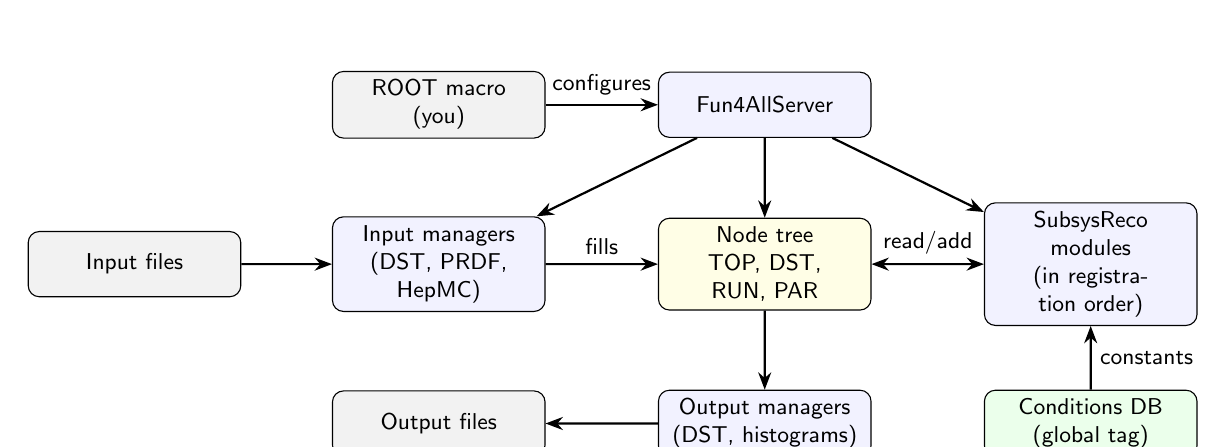
\begin{tikzpicture}[scale=0.92, transform shape, every node/.style={font=\small},
 box/.style={draw, rounded corners, text width=27mm, minimum height=9mm, align=center, fill=blue!5},
 arr/.style={-{Stealth[length=2.2mm]}, thick}]
\node[box, fill=gray!10] (macro) at (0.8,0) {ROOT macro\\(you)};
\node[box] (server) at (5.3,0) {Fun4AllServer};
\node[box, fill=gray!10] (files) at (-3.4,-2.2) {Input files};
\node[box] (in) at (0.8,-2.2) {Input managers\\(DST, PRDF, HepMC)};
\node[box, fill=yellow!10] (tree) at (5.3,-2.2) {Node tree\\TOP, DST, RUN, PAR};
\node[box] (mods) at (9.8,-2.2) {SubsysReco modules\\(in registration order)};
\node[box, fill=green!8] (cdb) at (9.8,-4.4) {Conditions DB\\(global tag)};
\node[box] (out) at (5.3,-4.4) {Output managers\\(DST, histograms)};
\node[box, fill=gray!10] (ofiles) at (0.8,-4.4) {Output files};
\draw[arr] (macro) -- node[above]{configures} (server);
\draw[arr] (server) -- (in); \draw[arr] (server) -- (tree); \draw[arr] (server) -- (mods);
\draw[arr] (files) -- (in);
\draw[arr] (in) -- node[above]{fills} (tree);
\draw[arr, {Stealth[length=2.2mm]}-{Stealth[length=2.2mm]}] (tree) -- node[above]{read/add} (mods);
\draw[arr] (tree) -- (out); \draw[arr] (out) -- (ofiles);
\draw[arr] (cdb) -- node[right]{constants} (mods);
\end{tikzpicture}
\caption{Schematic structure of a Fun4All job (own drawing). Modules communicate only through the node tree.}\label{fig:f4a}
\end{figure}

\subsection{The processing concept: a chain with snapshots}
All reconstruction and analysis is one chain of modules that could in principle run in a single job [S14].
In practice the chain is cut into stages, and the state of the node tree at the end of a stage is written to a file.
Such a file is called a \textbf{DST} (an old name, ``data summary tape'').
Reading the DST later and running the remaining modules gives the same result as running everything at once.
This has three benefits:
\begin{itemize}
\item Slow stages (for example tracking) run once, in a controlled production, and many users reuse their output.
\item Fast stages (for example your cluster-pair analysis) can be rerun many times on the saved output.
\item When a calibration changes, only the stages that depend on it need to be rerun.
\end{itemize}
Raw-data event combining (Section~\ref{sec:prod}) is the one step that always runs separately.

\conceptbox{Key idea}{A DST is not a ``file format'' in the usual sense. It is a frozen node tree.
The question ``what is in this DST?'' is answered by printing its node tree, not by opening a TBrowser.}

\subsection{The server's main loop}
Conceptually, \texttt{se->run(N)} does the following for each event:
\begin{enumerate}
\item Ask every input manager for the next event and synchronise them (Section~\ref{sec:sync}).
\item If a new run number appears, call \texttt{EndRun} for the old run and \texttt{InitRun} for the new run on every module.
\item Call \texttt{process\_event} on every registered module, in registration order.
\item Hand the tree to every output manager, which writes the selected nodes.
\item Call \texttt{ResetEvent} on the modules and reset the objects under the \texttt{DST} node.
\end{enumerate}
The order of modules is the order in which you registered them. Fun4All does not sort them by dependency; getting the order right is your job [S14].

%=====================================================================
\section{The node tree}\label{sec:nodetree}
%=====================================================================
\goal{Read a node-tree printout fluently and access any object in it.}

\subsection{Three kinds of node}
The node tree is the centre of the software, but it is mostly invisible to you [S14]. It is not a ROOT TTree.
It is built from three node classes in the \texttt{phool} package:
\begin{itemize}
\item \texttt{PHCompositeNode}: a directory that contains other nodes.
\item \texttt{PHDataNode}: holds any object, but cannot be written to a file.
\item \texttt{PHIODataNode}: holds an object that can be written to and read from a DST. The object must be ROOT-streamable.
\end{itemize}
Composite nodes and IO data nodes can be saved and restored. The structure of the tree is encoded in the branch names of the ROOT trees inside the DST.
A DST contains two ROOT trees: one with event-wise information and one with run-wise information [S14].
Not every object can be an IO node. Objects that wrap ACTS tracking classes, for example, cannot be streamed by ROOT and stay as plain data nodes.

\subsection{The standard layout}
\begin{figure}[h]\centering
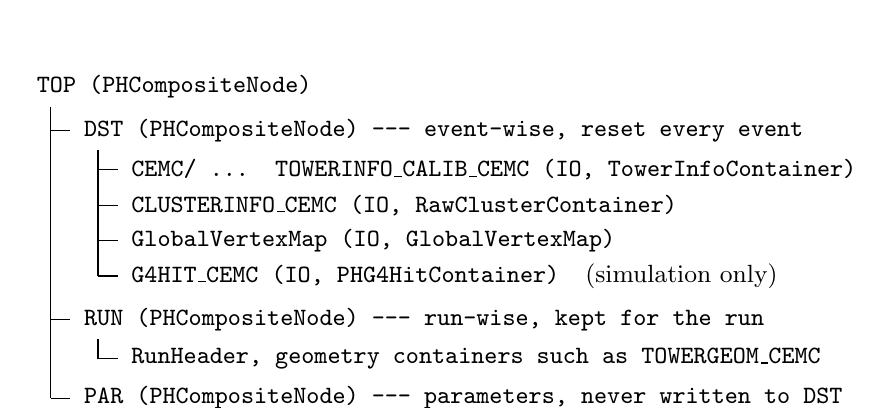
\begin{tikzpicture}[every node/.style={font=\small\ttfamily, anchor=west}, level distance=5mm]
\node (top) at (0,0) {TOP (PHCompositeNode)};
\node (dst) at (0.6,-0.55) {DST (PHCompositeNode) --- event-wise, reset every event};
\node at (1.2,-1.05) {CEMC/ ... TOWERINFO\_CALIB\_CEMC (IO, TowerInfoContainer)};
\node at (1.2,-1.50) {CLUSTERINFO\_CEMC (IO, RawClusterContainer)};
\node at (1.2,-1.95) {GlobalVertexMap (IO, GlobalVertexMap)};
\node at (1.2,-2.40) {G4HIT\_CEMC (IO, PHG4HitContainer) \ \rmfamily (simulation only)};
\node (run) at (0.6,-2.95) {RUN (PHCompositeNode) --- run-wise, kept for the run};
\node at (1.2,-3.45) {RunHeader, geometry containers such as TOWERGEOM\_CEMC};
\node (par) at (0.6,-3.95) {PAR (PHCompositeNode) --- parameters, never written to DST};
\draw (0.3,-0.25) -- (0.3,-3.95); \foreach \y in {-0.55,-2.95,-3.95} \draw (0.3,\y) -- (0.55,\y);
\draw (0.9,-0.8) -- (0.9,-2.40); \foreach \y in {-1.05,-1.50,-1.95,-2.40} \draw (0.9,\y) -- (1.15,\y);
\draw (0.9,-3.2) -- (0.9,-3.45); \draw (0.9,-3.45) -- (1.15,-3.45);
\end{tikzpicture}
\caption{Schematic node tree (own drawing). Node names are typical examples; print the tree of your own file to see the exact names.}\label{fig:tree}
\end{figure}
Figure~\ref{fig:tree} shows the layout. The meaning of the top-level nodes [S14]:
\begin{itemize}
\item \texttt{TOP}: the root of the default tree. Fun4All can manage several independent trees; embedding uses this (Section~\ref{sec:embed}).
\item \texttt{DST}: event-wise objects. Everything under it is reset after every event, which prevents information leaking from one event into the next.
You can choose which of its objects go into an output file. Sub-directories (one per detector) are saved and restored too.
\item \texttt{RUN}: run-wise objects (run header, geometry, run-level summaries). Not reset per event.
\item \texttt{PAR}: complicated parameter and geometry objects that should not be saved to a DST.
\end{itemize}
You may add your own composite node under \texttt{TOP}, but then resetting its contents is your responsibility.
Objects cannot be added to the \texttt{DST} node in the middle of a run, because that would make the output inconsistent.

\subsection{Printing the tree}
Every job prints the node tree when processing starts. You can also print it at any time from the macro:
{\footnotesize\begin{verbatim}
Fun4AllServer *se = Fun4AllServer::instance();
se->Print("NODETREE");
\end{verbatim}}
Each line gives the node name, whether it is an IO node, and the class of the stored object, for example
\texttt{G4HIT\_CEMC (IO,PHG4HitContainer)}. You need both the name and the class to fetch the object.

\subsection{Fetching an object}
The templated helper \texttt{findNode::getClass} (header \texttt{phool/getClass.h} in the current installation; some older examples include it through \texttt{fun4all/}) searches the tree below the node you pass:
{\footnotesize\begin{verbatim}
#include <calobase/TowerInfoContainer.h>
#include <phool/getClass.h>

int MyAna::process_event(PHCompositeNode *topNode)
{
  auto *towers = findNode::getClass<TowerInfoContainer>(topNode, "TOWERINFO_CALIB_CEMC");
  if (!towers)
  {
    std::cout << "TOWERINFO_CALIB_CEMC missing" << std::endl;
    return Fun4AllReturnCodes::ABORTRUN;
  }
  // ... loop over towers ...
  return Fun4AllReturnCodes::EVENT_OK;
}
\end{verbatim}}
\texttt{getClass} returns the first node with that name. If two nodes share a name (possible with several trees), you must search from the right top node [S14].

\subsection{Ownership}
Once you put an object on the tree, the tree owns it. Fun4All deletes the tree, and everything in it, at the end of the job.
Never \texttt{delete} an object you put on the tree. Deleting nodes during a job is not supported [S14].

\checksbox{\begin{itemize}
\item A \texttt{nullptr} from \texttt{getClass} almost always means a wrong node name, a missing input file, or a module registered in the wrong order.
\item Compare the class printed in the tree with the class in your template argument. Use the base class (Section~\ref{sec:schema}).
\end{itemize}}

%=====================================================================
\section{Your analysis module: the SubsysReco lifecycle}
%=====================================================================
\goal{Know exactly when each method of your module is called and what belongs in it.}

\subsection{The base class}
Every module derives from \texttt{SubsysReco} (\texttt{offline/framework/fun4all/SubsysReco.h}).
The base class provides default, do-nothing versions of all methods, so you only implement what you need [S14].

\begin{figure}[h]\centering
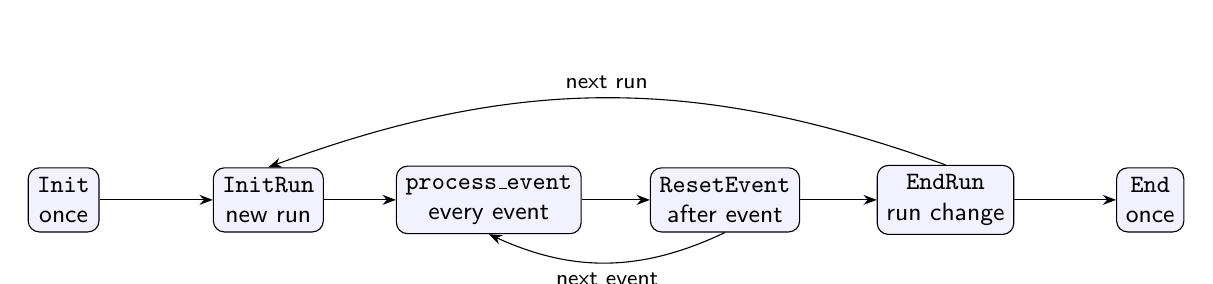
\begin{tikzpicture}[every node/.style={font=\small}, box/.style={draw, rounded corners, fill=blue!5, minimum height=7mm, align=center}]
\node[box] (init) at (0,0) {\texttt{Init}\\once};
\node[box] (ir) at (2.6,0) {\texttt{InitRun}\\new run};
\node[box] (pe) at (5.4,0) {\texttt{process\_event}\\every event};
\node[box] (re) at (8.4,0) {\texttt{ResetEvent}\\after event};
\node[box] (er) at (11.2,0) {\texttt{EndRun}\\run change};
\node[box] (end) at (13.8,0) {\texttt{End}\\once};
\draw[-{Stealth}] (init) -- (ir); \draw[-{Stealth}] (ir) -- (pe); \draw[-{Stealth}] (pe) -- (re);
\draw[-{Stealth}] (re.south) to[bend left=25] node[below]{\footnotesize next event} (pe.south);
\draw[-{Stealth}] (re) -- (er); \draw[-{Stealth}] (er) -- (end);
\draw[-{Stealth}] (er.north) to[bend right=20] node[above]{\footnotesize next run} (ir.north);
\end{tikzpicture}
\caption{Schematic call sequence of a \texttt{SubsysReco} module (own drawing).}\label{fig:life}
\end{figure}

\par\noindent\begin{tabularx}{\linewidth}{@{}lX@{}}\toprule
Method & When it is called and what belongs in it \\\midrule
\texttt{Init(topNode)} & Once, at registration or start of job. Book histograms, open output files, create your own output nodes. \\
\texttt{InitRun(topNode)} & Whenever data from a new run are seen. Load run-dependent calibrations, read geometry and run-level information. \\
\texttt{process\_event(topNode)} & Every event. Read objects, compute, fill histograms, store results on the tree. \\
\texttt{ResetEvent(topNode)} & After each event. Clear per-event containers that you own outside the \texttt{DST} node. \\
\texttt{EndRun(runnumber)} & Before \texttt{InitRun} of the next run. Caveat: the tree already holds the first event of the new run. \\
\texttt{End(topNode)} & Last call. Write and close files, print summaries. \\\bottomrule
\end{tabularx}
\smallskip

The caveat on \texttt{EndRun} matters: if you read run-level information from the tree inside \texttt{EndRun}, you may get the new run's values [S14].
Store what you need during the run instead.

\subsection{Return codes}
Each method returns an integer from \texttt{Fun4AllReturnCodes} (package \texttt{fun4all}). The most used values are:
\begin{itemize}
\item \texttt{EVENT\_OK}: continue normally.
\item \texttt{ABORTEVENT}: stop processing this event; later modules are not called for it, and it is not written out.
\item \texttt{DISCARDEVENT}: a positive code meaning the event should not be kept by the output (check the current source for the exact semantics in your build).
\item \texttt{ABORTRUN}: stop processing, typically used when a required node is missing. (\texttt{ABORTPROCESSING} also exists and ends the whole job.)
\end{itemize}
\texttt{ABORTEVENT} is how event selectors work: a module early in the chain that returns it acts as a filter for all later modules.

\subsection{Creating a module skeleton}
Do not copy and edit someone else's module. Use the generator script [S14]:
{\footnotesize\begin{verbatim}
mkdir -p ~/src/ClusterCounter && cd ~/src/ClusterCounter
CreateSubsysRecoModule.pl --all ClusterCounter
\end{verbatim}}
It creates \texttt{ClusterCounter.h}, \texttt{ClusterCounter.cc} with a print statement in every method, and, with \texttt{--all},
the build files \texttt{autogen.sh}, \texttt{configure.ac} and \texttt{Makefile.am}.
The generated build files do not contain the extra rules needed for new I/O classes (objects you want to write to a DST); for those you copy the pattern from an existing package.
A tutorial with a runnable macro is in the \texttt{tutorials} repository (\texttt{CreateSubsysRecoModule}).

\subsection{A minimal cluster counter}
The checkpoint exercise of this module asks for a module that prints cluster counts. Its essential part is:
{\footnotesize\begin{verbatim}
#include "ClusterCounter.h"
#include <calobase/RawCluster.h>
#include <calobase/RawClusterContainer.h>
#include <fun4all/Fun4AllReturnCodes.h>
#include <phool/getClass.h>
#include <TH1.h>

int ClusterCounter::Init(PHCompositeNode *)
{
  m_hN = new TH1F("hNclus", ";N clusters;events", 200, 0, 200);
  m_hE = new TH1F("hEclus", ";E_{clus} [GeV];clusters", 200, 0, 20);
  return Fun4AllReturnCodes::EVENT_OK;
}

int ClusterCounter::process_event(PHCompositeNode *topNode)
{
  auto *clus = findNode::getClass<RawClusterContainer>(topNode, m_nodeName);
  if (!clus) return Fun4AllReturnCodes::ABORTRUN;
  m_hN->Fill(clus->size());
  auto range = clus->getClusters();
  for (auto it = range.first; it != range.second; ++it)
  {
    m_hE->Fill(it->second->get_energy());
  }
  return Fun4AllReturnCodes::EVENT_OK;
}
\end{verbatim}}
Here \texttt{m\_nodeName} is a string member (for example \texttt{"CLUSTERINFO\_CEMC"}) with a setter, so the same module can count clusters from different builders.
The histograms are best handled by \texttt{Fun4AllHistoManager} or written in \texttt{End}.

\connectbox{Your \texttt{pi0EtaAnalysisPP24} module is exactly such a \texttt{SubsysReco}. Its \texttt{InitRun} is the right place for anything
run dependent (for example reading the trigger configuration or a per-run hot-tower map), and its \texttt{process\_event} reads
\texttt{TOWERINFO\_CALIB\_CEMC}, the cluster container and the vertex map. Check two things in your own code with the lifecycle in mind:
(i) nothing run dependent is read inside \texttt{EndRun}; (ii) any per-event buffers kept outside the \texttt{DST} node (for example the
photon list used for event mixing) are cleared or rotated deliberately, not by accident.}
%=====================================================================
\section{Schema evolution: why classes come in versions}\label{sec:schema}
%=====================================================================
\goal{Understand why you see \texttt{TowerInfov4} in a printout but should write \texttt{TowerInfoContainer} in your code.}

\subsection{What a file actually stores}
When ROOT writes a C++ object, it stores the \emph{data members}. The methods and the class layout come from the shared library loaded at read time [S14].
This has a consequence. Suppose version 1 of a class stored a time as a \texttt{short}, and you later change the member to a \texttt{float}.
Old files still contain a \texttt{short}. Reading them with the new library either fails or silently misinterprets the bytes.
The general rule follows: once a class has been written to files you want to keep, its data members must never change.

\subsection{The solution: a virtual base class with versioned implementations}
sPHENIX solves this with a pattern you will see everywhere [S14]:
\begin{enumerate}
\item An abstract base class (for example \texttt{TowerInfo}) declares the interface: virtual getters and setters, with default implementations that do nothing or return a sentinel.
\item Concrete versions (\texttt{TowerInfov1}, \texttt{TowerInfov2}, \dots) implement the interface with their own data members.
\item A new version is a new class. Old versions are kept in the library so that old files remain readable.
\item Analysis code uses only the base class. It calls \texttt{get\_energy()} and does not care which version is behind the pointer.
\end{enumerate}
Without the base class, every analysis would need a chain of ``if the file contains version 1, else if version 2, \dots'' branches.
With it, your code reads past, present and future data unchanged.

\subsection{Worked example: TowerInfo versions}
The calorimeter tower object illustrates the trade-offs [S15]:
\begin{itemize}
\item \texttt{v1} stores only the energy (amplitude).
\item \texttt{v2} stores full floating-point amplitude, time, pedestal, $\chi^2$ and status.
\item \texttt{v3} stores everything in \texttt{v2} plus the raw waveform samples (large; used for studies).
\item \texttt{v4} is the compact production version: amplitude, time packed as an integer with sub-sample precision, an 8-bit status word and a compressed $\chi^2$.
\end{itemize}
Each step trades disk space against information. Your code that calls \texttt{TowerInfo::get\_energy()} and \texttt{get\_time()} works for all of them.

\subsection{The catches}
\begin{itemize}
\item Adding a method to the base class does not add the data member to old versions. Your code must handle the default return value.
\item Never use public data members; always use methods.
\item Every version must stay compiled forever, and ROOT version changes can break old classes.
\item Never instantiate a versioned class in analysis code, except when you create a new object to store yourself [S14].
\end{itemize}

\pitfallbox{\begin{itemize}
\item Casting a base pointer to a specific version (for example \texttt{dynamic\_cast<TowerInfov2*>}) makes your code break on the next production. Use base-class methods.
\item A getter that returns a sentinel (often $0$ or NaN) because the version does not store that field is not a bug in the data. Zero-suppressed towers, for example, have no meaningful fit time or $\chi^2$ (Module 7).
\end{itemize}}

%=====================================================================
\section{Input and output managers}
%=====================================================================
\goal{Choose the right manager for each file type and understand event synchronisation.}

\subsection{Input managers}
An input manager opens files and places their content on the node tree. The main types are:
{\small\par\noindent\begin{tabularx}{\linewidth}{@{}>{\raggedright\arraybackslash}p{0.40\linewidth}X@{}}\toprule
Manager & Use \\\midrule
\texttt{Fun4AllDstInputManager} & Reads DSTs written by Fun4All; restores the node tree. The default for analysis. \\
\texttt{Fun4AllNoSyncDstInputManager} & Reads a DST without event synchronisation (for example a background file read in a different order). \\
\texttt{Fun4AllRunNodeInputManager} & Reads only the \texttt{RUN} node, for example geometry files fetched from the CDB. \\
\texttt{Fun4AllPrdfInputManager} & Reads raw PRDF files (raw-data level; normally only production and experts). \\
\texttt{Fun4AllHepMCInputManager} & Reads generator events in HepMC format (for example HIJING) for simulation. \\
\texttt{Fun4AllHepMCPileupInputManager} & Overlays several HepMC events to model pile-up. \\\bottomrule
\end{tabularx}}
\smallskip
Each manager takes either a single file (\texttt{AddFile}) or a text file with one file name per line (\texttt{AddListFile}).

\subsection{Synchronisation}\label{sec:sync}
You will often read two DSTs in parallel, for example calorimeter clusters from one file and the trigger or vertex information from another.
Fun4All guarantees that your modules see only complete, matching events [S14]:
\begin{itemize}
\item Every DST event stores its run number and event number (and, for simulation, the segment number).
\item The server compares these across all input managers for every event.
\item If they do not match, the event is skipped, and the next one is fetched.
\end{itemize}
A plain ROOT \texttt{TTree::AddFriend} cannot do this; it simply aligns entry numbers.
There is one trap. If two DST types are segmented differently (for example ten thousand events per file for one and a hundred thousand for the other), the segments you pair may contain no common events.
Fun4All will then read through all events without ever calling your \texttt{process\_event} [S14]. The fix is to build matching file lists, run by run.

\subsection{Output managers}
\texttt{Fun4AllDstOutputManager} writes the tree. By default it writes all nodes. You can restrict it with [S14]:
\begin{itemize}
\item \texttt{AddNode(name)} / \texttt{AddRunNode(name)}: write only these event-wise or run-wise nodes;
\item \texttt{StripNode(name)} / \texttt{StripRunNode(name)}: write everything except these.
\end{itemize}
You cannot mix ``add'' and ``strip'' calls on the same output manager.
Histograms are written separately, typically with a \texttt{Fun4AllHistoManager} or by your module in \texttt{End}.

\checksbox{\begin{itemize}
\item If a two-input job processes zero events, print run and event numbers from each file separately; the segments probably do not overlap.
\item After writing a DST, read it back with a one-module macro and print the node tree; the nodes you need must be there.
\end{itemize}}

%=====================================================================
\section{Macros: steering a job}
%=====================================================================
\goal{Read the big standard macros, and write small ones of your own.}

\subsection{What a macro is}
A Fun4All macro is a ROOT C++ macro (run with \texttt{root.exe -b -q 'Macro.C(args)'}). It loads libraries, creates the server,
registers modules and managers in order, runs, and ends. Libraries are loaded with \texttt{R\_\_LOAD\_LIBRARY(libfun4all.so)} at the top or \texttt{gSystem->Load(...)} inside.

\subsection{The standard macro and its helpers}
The \texttt{macros} repository holds \texttt{Fun4All\_G4\_sPHENIX.C}, which can do almost everything: run generators, read files, embed,
simulate any detector configuration, reconstruct, evaluate, run QA and your module. It cannot read raw data [S14].
The price is complexity. It is configured by many global flags defined in helper files under \texttt{macros/common}, for example:
\begin{itemize}
\item \texttt{Input::PYTHIA8}, \texttt{Input::SIMPLE}, \texttt{Input::GUN}, \texttt{Input::EMBED}, \texttt{Input::READHITS} (in \texttt{G4\_Input.C});
\item \texttt{Enable::CEMC}, \texttt{Enable::HCALIN}, \texttt{Enable::HCALOUT}, \texttt{Enable::MBD}, \texttt{Enable::CDB}, \texttt{Enable::DSTOUT};
\item helper functions such as \texttt{G4Init()}, \texttt{G4Setup()}, \texttt{CEMC\_Towers()}, \texttt{Process\_Calo\_Calib()}, \texttt{Jet\_Reco()}.
\end{itemize}
The flag \texttt{Input::READHITS} skips Geant4 and reads previously produced G4 hits, so that only the digitisation and reconstruction run again.

\subsection{A small custom macro}
For analysis, a short macro is clearer. The example below reads calibrated calorimeter DSTs and runs one module.
It is written for this text; adapt names to your files.
{\footnotesize\begin{verbatim}
#include <fun4all/Fun4AllServer.h>
#include <fun4all/Fun4AllDstInputManager.h>
#include <phool/recoConsts.h>
#include <clustercounter/ClusterCounter.h>
R__LOAD_LIBRARY(libfun4all.so)
R__LOAD_LIBRARY(libclustercounter.so)

void Fun4All_Count(int nEvents = 1000, const std::string &list = "dst_calo.list",
                   int runnumber = 0)
{
  Fun4AllServer *se = Fun4AllServer::instance();
  recoConsts *rc = recoConsts::instance();
  rc->set_StringFlag("CDB_GLOBALTAG", "<global tag>");   // see Section 8
  rc->set_uint64Flag("TIMESTAMP", runnumber);

  Fun4AllInputManager *in = new Fun4AllDstInputManager("DSTCALO");
  in->AddListFile(list);
  se->registerInputManager(in);

  auto *cc = new ClusterCounter("ClusterCounter");
  se->registerSubsystem(cc);

  se->run(nEvents);
  se->End();
  delete se;
  gSystem->Exit(0);
}
\end{verbatim}}
The same job could be expressed in \texttt{Fun4All\_G4\_sPHENIX.C} with \texttt{Input::READHITS}, a list file, and the module added in \texttt{G4\_User.C} [S14]; the small macro is easier to audit.

\subsection{Why stay inside Fun4All for analysis?}
It is tempting to write a quick ROOT loop over a flat tree instead. The school gives three reasons not to [S14]:
\begin{enumerate}
\item Many DSTs need further on-the-fly processing (recalibration, status flags, vertex corrections). These are \texttt{SubsysReco} modules and need the node tree.
\item With the data volumes of sPHENIX, analysis must eventually run in coordinated passes (the PHENIX ``analysis taxi'' model is planned), not as tens of thousands of private jobs.
\item CPU will become scarce once tracking production is in full use, so sharing passes matters.
\end{enumerate}
Producing a compact tree from a Fun4All module and then looping over that tree interactively remains good practice; the point is to start from the DST inside Fun4All.

%=====================================================================
\section{The conditions database (CDB)}\label{sec:cdb}
%=====================================================================
\goal{Get the right calibration for the right run, reproducibly.}

\subsection{Concepts}
Calibrations change with time: gains drift, towers die, alignments move. A conditions database stores such information with an \emph{interval of validity}.
Four words define the system:
\begin{itemize}
\item \textbf{Payload}: a file (often a ROOT file holding a \texttt{CDBTTree} or histograms) with the constants.
\item \textbf{Domain} (or type): the name of a kind of calibration, for example a tower-gain domain for the EMCal or the calorimeter geometry \texttt{calo\_geo}.
\item \textbf{Interval of validity (IOV)}: the range of timestamps for which a payload applies. In sPHENIX the timestamp is normally the run number.
\item \textbf{Global tag}: a named, frozen set of (domain, IOV, payload) assignments. Choosing a tag chooses a consistent set of calibrations for everything.
\end{itemize}
The sPHENIX CDB is a service with a PostgreSQL back end (the NPPS conditions database); payload files are served through CVMFS [S14].
Some calibrations still live outside the database, in the \texttt{calibrations} repository [S14].

\subsection{Using it from a macro}
Two flags on the \texttt{recoConsts} singleton select the calibrations for the whole job:
{\footnotesize\begin{verbatim}
recoConsts *rc = recoConsts::instance();
rc->set_StringFlag("CDB_GLOBALTAG", tag);       // which frozen set
rc->set_uint64Flag("TIMESTAMP", runnumber);     // which IOV
\end{verbatim}}
A module then asks for the payload of a domain:
{\footnotesize\begin{verbatim}
std::string url = CDBInterface::instance()->getUrl("<domain name>");
CDBTTree *cdbt = new CDBTTree(url);
cdbt->LoadCalibrations();
float g = cdbt->GetFloatValue(channel, "<field name>");
\end{verbatim}}
\texttt{CDBInterface} lives in the \texttt{ffamodules} package and \texttt{CDBTTree} in \texttt{cdbobjects}.
The standard calorimeter calibration macro \texttt{Calo\_Calib.C} uses exactly this mechanism to fetch the geometry, the hot-tower maps and the gains (Module 7).
Many modules also accept a ``direct URL'' (a file path) that bypasses the database, which is useful for testing a new calibration before it is in a tag.

\subsection{Why tags and not ``the latest''}
Using the most recent constants sounds attractive, but it makes results irreproducible: two people running a week apart would get different answers.
A frozen tag makes the processing a pure function of (code version, tag, input files).
Production names its outputs after the build and the tag for this reason.

\pitfallbox{\begin{itemize}
\item Forgetting \texttt{TIMESTAMP}: you get constants for the wrong IOV, or none at all.
\item Different tags for data and simulation: both may be correct in themselves, but data/MC comparisons then mix different energy scales or status maps. Record the tag of every sample in your analysis note.
\item Overriding one domain with a direct URL and forgetting it there. Print all direct URLs at job start.
\end{itemize}}

\connectbox{Your data chain applies the tower calibration and status maps from the data global tag through \texttt{Calo\_Calib}-style processing,
while your efficiency simulation used a simulation tag and the official simulation calibration chain. That is the normal arrangement, but it
means every data/MC comparison (peak positions, widths, hot-tower acceptance) has to be read with the two tags in mind. A good habit is a
one-line header in each output file with the build, the global tag and the timestamp used.}

%=====================================================================
\section{Building and installing your code}
%=====================================================================
\goal{Build a package into a private install area and use it, without clashing with the central builds.}

\subsection{The repositories}
The main public repositories of the sPHENIX collaboration on GitHub are [S14]:
{\small\par\noindent\begin{tabularx}{\linewidth}{@{}>{\raggedright\arraybackslash}p{0.25\linewidth}X@{}}\toprule
Repository & Content \\\midrule
\texttt{coresoftware} & All framework, simulation, reconstruction and calibration code (\texttt{offline/framework}, \texttt{offline/packages}, \texttt{simulation/g4simulation}, \dots). \\
\texttt{online\_distribution} & Raw-data format and decoding software. \\
\texttt{macros} & Standard macros, including \texttt{macros/common} and detector configurations. \\
\texttt{calibrations} & Calibration files kept outside the database. \\
\texttt{analysis} & User analysis packages (yours can live here). \\
\texttt{tutorials} & Worked tutorials, including module creation and calorimeter data analysis. \\\bottomrule
\end{tabularx}}

\subsection{Builds and the setup script}
The central software is installed in several builds [S14]:
\texttt{new} (daily build of the current code), \texttt{ana} (weekly archival builds, numbered, for example \texttt{ana.<N>}),
\texttt{play} (testing new external versions), \texttt{debug} (no optimisation), \texttt{clang} and an instrumented build for run-time checking.
You select one with the setup script:
{\footnotesize\begin{verbatim}
source /opt/sphenix/core/bin/sphenix_setup.sh -n ana.<N>
\end{verbatim}}
Daily builds roll over after a few days. If you build against \texttt{new}, your private libraries can become inconsistent with the central ones within days.
For long projects, pin a fixed \texttt{ana} build and update deliberately [S14].

\subsection{Autotools: source, build and install areas}
sPHENIX packages use autoconf/automake. Keep three areas separate [S14]:
{\footnotesize\begin{verbatim}
# once per package
mkdir -p $HOME/build/ClusterCounter && cd $HOME/build/ClusterCounter
$HOME/src/ClusterCounter/autogen.sh --prefix=$MYINSTALL
make -j4 install
# in every new shell (after sphenix_setup)
source $OPT_SPHENIX/bin/setup_local.sh $MYINSTALL
\end{verbatim}}
Here \texttt{MYINSTALL} is a variable you define, for example \texttt{\$HOME/install}.
\texttt{autogen.sh} must be called with the full path to the source, so that debuggers can find the source files.
The \texttt{setup\_local.sh} script prepends your install area to the library and include paths; ROOT~6 needs this to find your headers [S14].
Each package is built on its own, so you rebuild only what you change.

\subsection{Coding conventions}
Code lives long and is maintained by others. The software coordinators ask for: comments (they cost nothing at run time), simple code over clever code,
and adherence to the coding conventions on the wiki, increasingly checked with \texttt{clang-tidy} [S14].
They also warn that machine-generated code tends to be over-complicated for this environment.

\subsection{Outside SDCC}
The software is also mirrored on a public CVMFS repository (\texttt{/cvmfs/sphenix.opensciencegrid.org}), and Singularity/Docker containers with the farm image exist [S14].
These are useful for development on a laptop, but data access and batch resources require SDCC.

\pitfallbox{\begin{itemize}
\item Forgetting \texttt{setup\_local.sh} in a new shell or batch script: ROOT silently loads the central library of the same name, or fails to find yours.
\item Building against \texttt{new} and running a week later: undefined-symbol errors or subtle mismatches. Pin an \texttt{ana} build.
\item Committing autotools-generated files (\texttt{Makefile.in}, \texttt{configure}) from the source area. Build out of source.
\end{itemize}}

%=====================================================================
\section{Production, file catalogs and batch jobs}\label{sec:prod}
%=====================================================================
\goal{Know how official DSTs are made and how to find and process them responsibly.}

\subsection{The production chain}\label{sec:filecat}
Raw data arrive as one PRDF file stream per readout computer (per SEB, EBDC, MVTX or INTT server) [S13].
Production then runs a sequence of Fun4All passes [S14]:
\begin{enumerate}
\item \textbf{Event combining}: the per-computer streams are aligned using the beam-clock counter, so that ``event $n$'' in the output comes from one bunch crossing.
For streaming detectors (INTT, MVTX, TPC), hits are associated with a triggered crossing within a small window of beam-clock counts.
\item \textbf{Calorimeter reconstruction}: waveform fitting to towers (the DST you use, \texttt{DST\_CALOFITTING}, is the output of this step), and further calorimeter products.
\item \textbf{Global reconstruction}: trigger, MBD vertex and timing, sEPD and ZDC information.
\item \textbf{Tracking}: clustering per detector, then seeding and fitting in more than one pass, with TPC distortion corrections derived from histograms aggregated over many files in between (Module 8).
\end{enumerate}
Each pass reads the previous DSTs and writes new ones; the chain is a direct application of the ``snapshot'' concept of Section~2.

\subsection{Finding files}
All official files are registered in the file catalog; you do not need to know their paths [S14].
Use the provided scripts instead of listing Lustre:
\begin{itemize}
\item \texttt{CreateDstList.pl}: produces, for a DST type, per-run lists of files that can be fed directly to \texttt{AddListFile}.
\item \texttt{CreateFileList.pl}: the equivalent for official simulation productions; run without arguments to see the available sample types and options.
It first deletes existing list files in the directory so that you cannot mix samples by accident [S14].
\end{itemize}

\subsection{Run information}
The DAQ database records, for each run, which subsystems were included, which triggers were enabled, their scaledowns, and the trigger names [S13].
Trigger names and bit assignments changed within data-taking periods, especially in 2024, so always look them up per run rather than assuming a fixed map [S13].
Inside Fun4All you can decode the GL1 trigger words yourself, or use the \texttt{TriggerAnalyzer} helper (package \texttt{calotrigger}), which knows the names (Module 5).

\subsection{Batch jobs: the rules that protect everyone}
You will process data on the HTCondor farm. The school was explicit about good practice [S14]:
\begin{itemize}
\item Submit from an sPHENIX interactive node; this determines which pool you use.
\item The executable is a shell script that sets up the environment itself (\texttt{source .../sphenix\_setup.sh -n <build>}, then \texttt{setup\_local.sh}), prints the environment for debugging, and runs \texttt{root.exe -b -q}.
\item Never use \texttt{GetEnv = True}: it copies your interactive environment into the job and makes behaviour unpredictable.
\item Set \texttt{Notification = Never}; thousands of mails can get the account blocked.
\item Request realistic memory (\texttt{request\_memory}); simulation jobs need more than the default. Too little gets jobs evicted; far too much blocks the farm.
\item Do not let evicted jobs restart automatically (a periodic-hold expression is recommended); they will usually fail again.
\item Write the condor log to local disk of the submit host, and job outputs to \texttt{/sphenix/user} or Lustre, never to \texttt{/tmp} on a farm node.
\item Keep logs short: per-event printouts from thousands of jobs slow the shared disks.
\item Do not reuse inherited job files without understanding them.
\end{itemize}

\connectbox{Your pass-1 and pass-2 workflow is a two-stage version of the production chain: pass 1 is a Fun4All job over \texttt{DST\_CALOFITTING}
that writes per-run histograms and trees; pass 2 merges and loops over them. The two habits that matter most are the ones in this section:
build file lists with the catalog tools, run by run, and pin one \texttt{ana} build for the whole pass. If you ever need to combine a calorimeter
DST with another DST type (for example a tracking product), check that the segments overlap before launching jobs.}
%=====================================================================
\section{Detector simulation with Geant4}
%=====================================================================
\goal{Understand what Geant4 computes, how sPHENIX wraps it, and what a G4Hit contains.}

\subsection{Why simulate the detector at all}
Every measured spectrum is the true spectrum folded with the detector: acceptance, efficiency, resolution, and biases.
To unfold these effects you need a model of the detector that you trust. Monte Carlo simulation provides it:
generate events with known truth, pass them through a faithful model of the material and the readout, reconstruct them exactly like data,
and compare reconstructed with true quantities. Your $\pi^0$ reconstruction efficiency is exactly such a ratio.

\subsection{What Geant4 does: particle transport in steps}
Geant4 [R1] propagates each particle through the geometry one \emph{step} at a time [S14].
The step length is set by two things: the physics processes and the geometry boundaries.
\begin{itemize}
\item \textbf{Discrete processes} (for example pair conversion, Compton scattering, hadronic interactions) occur at random points.
For a process with mean free path $\lambda$, the probability to travel a distance $x$ without interacting is $P(x)=e^{-x/\lambda}$.
Geant4 samples the next interaction point for each process from this law and takes the shortest.
\item \textbf{Continuous processes} (ionisation energy loss, multiple scattering) act along every step. Energy loss follows the Bethe formula
for heavy charged particles, $-\langle dE/dx\rangle \propto z^2 (Z/A)\beta^{-2}[\ln(\ldots)-\beta^2-\ldots]$, with a minimum near $\beta\gamma\approx3$--$4$ (the ``minimum ionising particle'').
\item \textbf{Boundaries}: a step ends when the particle leaves a volume, so that each step lies in exactly one material.
\end{itemize}
To keep the CPU finite, secondaries below a \emph{production threshold} (specified as a range, converted to an energy per material) are not created; their energy is deposited locally.
A \emph{physics list} chooses which models describe each process in each energy range. Hadronic showers are the least certain part of any simulation,
which is why the calorimeter test-beam comparison in Section~\ref{sec:validate} matters.

\subsection{Electromagnetic showers in one paragraph}
A high-energy photon converts into an $e^+e^-$ pair after about $\frac{9}{7}X_0$, where $X_0$ is the radiation length.
Electrons radiate bremsstrahlung photons, which convert again, and the particle number roughly doubles every $X_0$ until the energies fall to the critical energy $E_c$,
below which ionisation dominates. The depth of the shower maximum is
\begin{equation}
t_{\max} \approx \ln\!\left(\frac{E}{E_c}\right) + C, \qquad C\approx -0.5 \text{ (electrons)}, \ +0.5 \text{ (photons)},
\end{equation}
in units of $X_0$. The lateral size is set by the Moli\`ere radius $R_M$; about 90\% of the energy lies within one $R_M$ of the axis.
\textbf{Worked example.} For tungsten, $E_c\approx 8$~MeV. A 4~GeV photon then has $t_{\max}\approx\ln(500)+0.5\approx 6.7\,X_0$.
The sPHENIX EMCal is about 18 radiation lengths deep (design value [R5]), so such a shower is well contained longitudinally.
The EMCal towers ($\Delta\eta\times\Delta\phi\approx0.025\times0.025$) are comparable to $R_M$, so a photon shares energy among a few towers, which is what clustering exploits (Module 7).

\subsection{Sampling calorimeters and the sampling fraction}
In a sampling calorimeter only the active material (scintillating fibres in the EMCal, scintillator tiles in the HCal) produces signal.
The \emph{sampling fraction} is
\begin{equation}
f_{\mathrm{samp}} = \frac{E_{\mathrm{active}}}{E_{\mathrm{active}}+E_{\mathrm{absorber}}}.
\end{equation}
Geant4 records energy in both active and absorber volumes (sPHENIX keeps separate hit containers such as \texttt{G4HIT\_CEMC} and \texttt{G4HIT\_ABSORBER\_CEMC} [S14]).
The calibration constant that maps active energy to shower energy is, to first order, $1/f_{\mathrm{samp}}$.
Fluctuations of the sampled fraction are the main source of the stochastic term $a/\sqrt{E}$ in the energy resolution
$\sigma_E/E = a/\sqrt{E}\oplus b$ (Module 3).
Scintillator light output is not exactly proportional to deposited energy at high ionisation density; Birks' law,
$dL/dx = S\,(dE/dx)/(1+k_B\,dE/dx)$, is the standard model, and the simulation can store a light-yield-weighted energy in addition to the raw deposit.

\subsection{Charged particles in the solenoid field}
In a uniform field $B$, a particle of charge $e$ and transverse momentum $p_T$ moves on a circle of radius
\begin{equation}
R\,[\mathrm{m}] = \frac{p_T\,[\mathrm{GeV}/c]}{0.3\,B\,[\mathrm{T}]}.
\end{equation}
\textbf{Worked example.} With the 1.4~T sPHENIX solenoid, a 1~GeV/$c$ track has $R=1/(0.3\times1.4)\approx2.4$~m.
Over the TPC lever arm (outer radius about 0.8~m) such a track bends visibly; a 10~GeV/$c$ track much less, which is why momentum resolution degrades with $p_T$ (Module 8).
In simulation the field is not uniform: a three-dimensional field map is used, fetched like a calibration (the standard macros refer to field-map payloads in the CDB).

\subsection{How sPHENIX wraps Geant4: PHG4Reco}
Geant4 runs inside Fun4All as one module, \texttt{PHG4Reco} [S14]. Its job in the chain is:
\begin{enumerate}
\item In \texttt{Init}, build the world volume, construct each enabled detector subsystem, set the field, and initialise Geant4.
\item In \texttt{process\_event}, take the generated particles from the node tree (the \texttt{PHG4INEVENT} node), transport them, and fill hit containers.
\end{enumerate}
Each detector is a self-contained subsystem configured from the macro [S14]. Generic shapes (\texttt{PHG4CylinderSubsystem}, boxes, cones) exist for quick studies;
the real detectors have their own subsystems (for example \texttt{PHG4SpacalSubsystem} for the EMCal, \texttt{PHG4IHCalSubsystem} and \texttt{PHG4OHCalSubsystem} for the HCals).
A notable design choice: there is no deep volume hierarchy; detectors are placed directly in the world volume.
A ``black hole'' volume around the detector absorbs everything that leaves, so that CPU is not spent on particles that cannot come back.

\subsection{G4Hits and truth}
After every step, Geant4 calls a user stepping action with full information about the step [S14].
sPHENIX stepping actions build \textbf{G4Hits}: for each particle crossing an active volume they sum the energy loss and store entry and exit positions and times,
plus subsystem-specific quantities such as ionisation energy or light yield [S14].
The \textbf{truth} record (\texttt{PHG4TruthInfoContainer}) keeps the generated particles and their ancestry, so that every hit can be traced back to a primary.
To save space, secondaries that neither leave hits nor are ancestors of a particle with hits are dropped [S14].

\subsection{From hits to towers: digitisation}
Hits are energies in active volumes, not detector signals. Digitisation turns them into what the electronics would record:
\begin{enumerate}
\item Hits are grouped into cells and towers using the detector geometry (for the EMCal, cell reconstruction for the projective spacal geometry, then tower building).
\item The tower energy is converted to a signal: in the current chain, \texttt{CaloWaveformSim} produces a sampled waveform with a pulse template, pedestal and noise.
\item The \emph{same} waveform fitting (\texttt{CaloTowerBuilder}) and calibration modules used for data then produce \texttt{TowerInfo} objects.
\end{enumerate}
The principle is ``common reconstruction for raw and simulated data'' [S14]: once you are past digitisation, data and simulation go through identical code.
This is what makes efficiency corrections meaningful. Effects that the digitisation does not model (for example a sensor nonlinearity, or a hot tower) must be added explicitly or corrected for (Module 7).

\begin{figure}[h]\centering
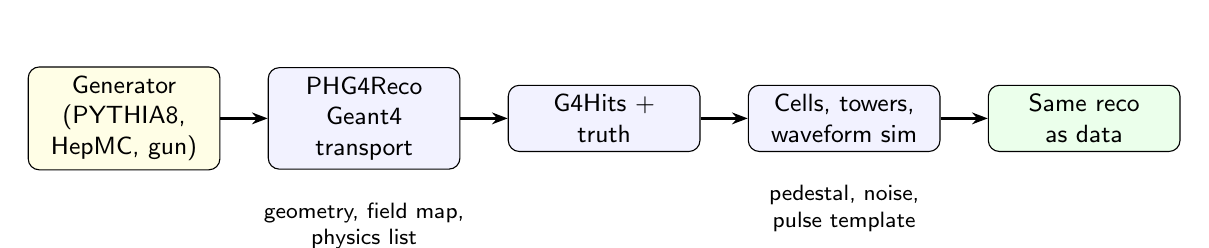
\begin{tikzpicture}[node distance=4mm and 6mm, every node/.style={font=\small},
 box/.style={draw, rounded corners, minimum height=8mm, align=center, fill=blue!5, text width=22mm},
 arr/.style={-{Stealth[length=2mm]}, thick}]
\node[box, fill=yellow!10] (gen) {Generator\\(PYTHIA8, HepMC, gun)};
\node[box, right=of gen] (g4) {PHG4Reco\\Geant4 transport};
\node[box, right=of g4] (hits) {G4Hits +\\truth};
\node[box, right=of hits] (digi) {Cells, towers,\\waveform sim};
\node[box, right=of digi, fill=green!8] (reco) {Same reco\\as data};
\draw[arr] (gen) -- (g4); \draw[arr] (g4) -- (hits); \draw[arr] (hits) -- (digi); \draw[arr] (digi) -- (reco);
\node[below=3mm of g4, font=\footnotesize, text width=40mm, align=center] {geometry, field map,\\physics list};
\node[below=3mm of digi, font=\footnotesize, text width=40mm, align=center] {pedestal, noise,\\pulse template};
\end{tikzpicture}
\caption{Schematic simulation chain (own drawing).}\label{fig:simchain}
\end{figure}

\subsection{Adding your own detector}
A new Geant4 detector needs three classes [S14]: a \emph{Subsystem} (the interface to Fun4All), a \emph{Detector} (builds the volumes),
and a \emph{SteppingAction} (makes hits). Optional classes handle parameters and display.
The script \texttt{CreateG4Subsystem.pl} generates a template, and the \texttt{g4exampledetector} repository contains a worked example [S14].
You will rarely need this, but it shows how the official detectors are built.

\checksbox{\begin{itemize}
\item For a single photon gun, the sum of active plus absorber G4Hit energy in the calorimeters should be close to the photon energy; the active part divided by the total is the sampling fraction.
\item The number of truth particles per event should match what the generator produced, plus kept secondaries.
\item Simulation is slow: test with 10 events, measure the time per event, then plan the batch.
\end{itemize}}

%=====================================================================
\section{Event generators}
%=====================================================================
\goal{Choose and configure the generator that matches the physics question.}

\subsection{The menu}
Fun4All interfaces several generators [S14]: PYTHIA8 (and PYTHIA6), HIJING through HepMC files, generic HepMC2 or OSCAR input,
single-particle generators, and special generators for $\Upsilon$ and $D^0$. The table summarises which to use when.

{\small\par\noindent\begin{tabularx}{\linewidth}{@{}>{\raggedright\arraybackslash}p{0.40\linewidth}X@{}}\toprule
Generator / module & Typical use \\\midrule
\texttt{PHPythia8} & $p$+$p$ events: minimum bias, jets, prompt photons. Configured by a PYTHIA card file (\texttt{set\_config\_file}). \\
HIJING via \texttt{Fun4AllHepMCInputManager} & Heavy-ion background (Au+Au, O+O) for occupancy, underlying event, embedding. \\
\texttt{PHG4SimpleEventGenerator} & One or more particles of a chosen species with flat $p_T$ (or $p$), $\eta$ and $\phi$ ranges. Efficiency studies. \\
\texttt{PHG4ParticleGun}, \texttt{PHG4ParticleGenerator} & Fixed or simple-distribution guns for detector studies. \\
\texttt{PHG4ParticleGeneratorVectorMeson}, \texttt{...D0} & Quarkonia and charm decays. \\
\texttt{Fun4AllHepMCPileupInputManager}, \texttt{PHG4PileupGenerator} & Add pile-up collisions to a signal event. \\\bottomrule
\end{tabularx}}

\subsection{PYTHIA8 for p+p}
PYTHIA [R2] generates a hard scattering from parton distributions and matrix elements, then adds initial- and final-state showers,
multiple parton interactions and hadronisation. Two practical points matter for cross-section work:
\begin{itemize}
\item \textbf{Hard-scale binning.} Minimum-bias PYTHIA produces very few high-$p_T$ $\pi^0$s. Samples are therefore generated in bins of the hard-scattering scale $\hat{p}_T$,
or filtered with a trigger (for example \texttt{PHPy8JetTrigger}, used in the standard embedding macro, accepts events with a jet above a threshold).
Each bin $i$ must be weighted by $w_i=\sigma_i/N_i$, the generator cross section of the bin divided by the number of generated events, before combining.
\item \textbf{Tune.} The parameters of the non-perturbative models are tuned to data. sPHENIX simulations commonly use a PYTHIA8 tune adapted to RHIC energies (the ``Detroit'' tune).
\end{itemize}

\subsection{Single-particle guns}
A single-particle gun places one known particle per event. The pattern is:
{\footnotesize\begin{verbatim}
auto *gen = new PHG4SimpleEventGenerator();
gen->add_particles("pi0", 1);
gen->set_vertex_distribution_function(PHG4SimpleEventGenerator::Gaus,
          PHG4SimpleEventGenerator::Gaus, PHG4SimpleEventGenerator::Gaus);
gen->set_vertex_distribution_mean(0., 0., 0.);
gen->set_vertex_distribution_width(0., 0., 20.);   // cm, choose to match data
gen->set_eta_range(-1.2, 1.2);
gen->set_phi_range(-M_PI, M_PI);
gen->set_pt_range(1., 20.);
se->registerSubsystem(gen);
\end{verbatim}}
In \texttt{Fun4All\_G4\_sPHENIX.C} the same object is reached through \texttt{Input::SIMPLE = true} and \texttt{INPUTGENERATOR::}\allowbreak\texttt{SimpleEventGenerator[0]}.
A gun with flat $p_T$ samples all $p_T$ evenly, which gives good statistics everywhere but the wrong spectrum shape.
Because efficiency in a bin depends on the spectrum within the bin (through resolution and bin migration), the gun sample must be reweighted to a realistic spectrum before computing efficiencies.

\subsection{Beam parameters and vertex}
The collision vertex in data is spread along $z$ by tens of centimetres and depends on the crossing angle and the run period.
The macros provide a helper, \texttt{Input::ApplysPHENIXBeamParameter}, which sets the vertex distribution and beam crossing for a chosen beam configuration
(for example \texttt{Input::pp\_COLLISION} or \texttt{Input::AA\_COLLISION}, selected with \texttt{Input::BEAM\_CONFIGURATION}).
The simulated vertex distribution should match the data after your vertex cut; otherwise acceptance at the edges of $|\eta|<1.1$ is biased.

\connectbox{Your efficiency simulation uses a $\pi^0$/$\eta$ gun with flat $p_T$, Hagedorn-type reweighting and an extra cluster-level smearing.
Three checks follow from this section: (i) the gun $\eta$ range must be wider than the EMCal acceptance, so that edge migration is modelled;
(ii) the reweighting must be applied before forming the efficiency ratio, not after; (iii) the simulated $z$-vertex distribution must cover your
vertex cut with the shape seen in the triggered data, or the efficiency must be computed in $z$-vertex bins. For Au+Au $R_{CP}$, the efficiency also
depends on centrality through cluster overlap, which is exactly what embedding (next section) is for.}

%=====================================================================
\section{Embedding}\label{sec:embed}
%=====================================================================
\goal{Understand sim-into-sim and sim-into-data embedding and their pitfalls.}

\subsection{Why embed}
A particle in an empty detector is reconstructed under ideal conditions. In a real event it shares the calorimeter with the underlying event, other particles and noise.
Clusters overlap, isolation energies grow, and energy is added to or removed from your object.
\textbf{Embedding} places a simulated signal into a realistic background event, so that the reconstruction sees realistic occupancy.
The efficiency is then the fraction of embedded particles that are recovered, with the background effects included.

\subsection{Two kinds}
\begin{itemize}
\item \textbf{Sim into sim.} The background is itself simulated (for example HIJING Au+Au events, or minimum-bias PYTHIA for $p$+$p$).
In the standard macros, \texttt{Input::EMBED = true} reads a previously simulated background DST, and the new signal is simulated and merged into it.
The background vertex must be reused for the signal, so that both come from the same point (\texttt{set\_reuse\_existing\_vertex} on the generator).
\item \textbf{Sim into data.} The background is a real data event. The calorimeter towers of the simulated signal, digitised consistently, are added to the data towers.
The \texttt{caloembedding} package contains the tools: \texttt{caloTowerEmbed} adds simulated towers to data towers, \texttt{CombineTowerInfo} merges two tower containers,
and \texttt{HepMCCollisionVertex} takes the data vertex so that the signal can be generated at the same position.
This uses two node trees at once: one top node holds the data event, the other the simulation [S14].
\end{itemize}

\begin{figure}[h]\centering
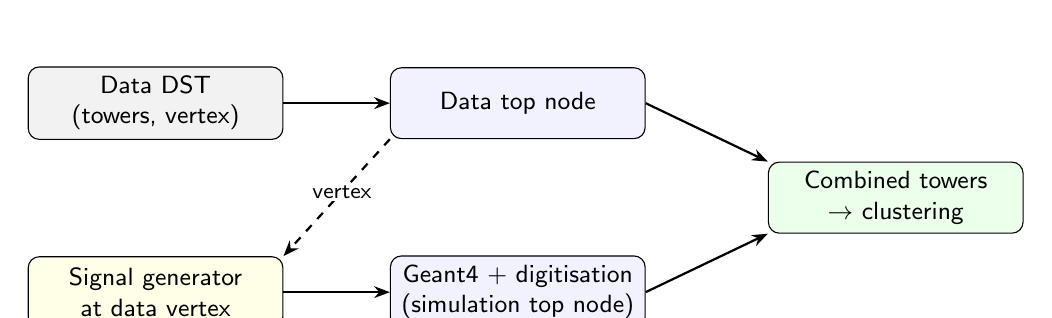
\begin{tikzpicture}[every node/.style={font=\small},
 box/.style={draw, rounded corners, minimum height=9mm, align=center, fill=blue!5, text width=30mm},
 arr/.style={-{Stealth[length=2mm]}, thick}]
\node[box, fill=gray!10] (data) at (0,0) {Data DST\\(towers, vertex)};
\node[box] (dtree) at (4.6,0) {Data top node};
\node[box, fill=yellow!10] (gen) at (0,-2.4) {Signal generator\\at data vertex};
\node[box] (sim) at (4.6,-2.4) {Geant4 + digitisation\\(simulation top node)};
\node[box, fill=green!8] (comb) at (9.4,-1.2) {Combined towers\\$\rightarrow$ clustering};
\draw[arr] (data) -- (dtree); \draw[arr] (gen) -- (sim);
\draw[arr] (dtree.east) -- (comb.north west); \draw[arr] (sim.east) -- (comb.south west);
\draw[arr, dashed] (dtree.south west) -- node[pos=0.45, fill=white, inner sep=1pt, font=\footnotesize]{vertex} (gen.north east);
\end{tikzpicture}
\caption{Schematic sim-into-data embedding with two node trees (own drawing).}\label{fig:embed}
\end{figure}

\pitfallbox{\begin{itemize}
\item Vertex mismatch: a signal generated at $z=0$ embedded into an event at $z=+25$~cm points to the wrong towers. Always take the background vertex.
\item Calibration mismatch: in sim-into-data, the simulated towers must be on the same energy scale as the data towers; otherwise the merged cluster energy is biased.
\item Status mismatch: hot or dead towers masked in data must be treated the same way for the embedded signal, or the efficiency near bad towers is wrong.
\item Double counting: the background event already contains real particles of the same species; truth matching must identify the embedded one.
\end{itemize}}

\connectbox{In your Au+Au $R_{CP}$ work the efficiency for central events is lower than for peripheral events because of cluster overlap and the
underlying event; embedding into HIJING or into data is the standard way to measure this centrality dependence. In $p$+$p$ the occupancy is low, so
embedding into minimum-bias PYTHIA mainly checks the effect of pile-up and of the vertex. If your efficiency gun was embedded into PYTHIA events,
remember that the background's own hot-tower treatment (absent in simulation) is not the data's, so apply the data hot-tower mask to the simulation explicitly.}
%=====================================================================
\section{Is the simulation right? A worked validation case}\label{sec:validate}
%=====================================================================
\goal{Learn how to validate a simulation against data, using the calorimeter test-beam re-analysis presented at the workfest [S47].}

\subsection{The question}
The jet energy scale in sPHENIX is calibrated with simulation, then checked in situ with photon--jet balance (Module 7).
Any difference between the true and the simulated response of the calorimeters to single hadrons propagates into the jet energy scale.
The calorimeter prototypes were tested in hadron and electron beams at Fermilab in 2016--2018, and the 2016 results are public [R4].
The workfest study [S47] asked: does the current sPHENIX Geant4 description reproduce those beam data, and what uncertainty should be assigned?

\subsection{Lesson 1: know exactly what a published figure shows}
A careful reading of the published analysis code showed that, in the resolution plots, the measured energy distribution in each beam-energy bin
had been rescaled so that its mean sat exactly at the beam energy, separately for data and for simulation [S47].
Such a figure tests only the \emph{shape} (the resolution); it says nothing about linearity or about the data-to-simulation energy scale.
The linearity figures, in contrast, used one scale factor for all energies, so they do show the genuine nonlinearity.
\emph{General rule:} before comparing to a published plot, find out what normalisation was applied.

\subsection{Lesson 2: combine layers the same way in data and simulation}
The total hadron energy is a weighted sum of the layers, $E = c\,[\,g\,E_{\mathrm{EMCal}} + w\,E_{\mathrm{IHCal}} + E_{\mathrm{OHCal}}\,]$.
The study found that the original analysis had used different inner-HCal weights $w$ for data and simulation [S47].
Using the same weight in both is the only apples-to-apples comparison; with it, the simulated resolution came out slightly better than the data.
A simulation that is ``too good'' is common: real detectors have non-uniformities, dead channels and noise that a simulation omits unless they are added.

\subsection{Lesson 3: reproduce the geometry that was actually in the beam}
Two different inner-HCal prototypes existed. The first attempt to resurrect the old simulation used the wrong one;
the error was found by comparing G4 hits, event by event, between the archived and the new simulation [S47].
\emph{General rule:} validate at the lowest level (G4 hits) before comparing reconstructed quantities.

\subsection{Lesson 4: the beam is not pure}
At the lowest beam momenta, the beam contained muons and other contaminants that neither the original nor the new simulation included [S47].
Those points should be excluded or modelled. The same logic applies to collision data: a simulation of pure signal cannot describe a data sample with background.

\subsection{Lesson 5: turn the comparison into an uncertainty}
The proposed procedure [S47] has two parts:
\begin{enumerate}
\item Fit the data-to-simulation ratio of the single-hadron response as a function of energy in the full (EMCal+IHCal+OHCal) configuration,
and propagate it to jets by reweighting the energies of the hadronic constituents of simulated anti-$k_T$ jets. Photons from $\pi^0$ decays are not affected,
because the electromagnetic response is constrained separately.
\item Because the real inner HCal differs from the steel prototype (different structure, hence different leakage), simulate the actual sPHENIX configuration and vary the leakage generously, taking the change as an additional uncertainty.
\end{enumerate}
The result is an energy-dependent single-hadron uncertainty that adds to the in situ photon--jet constraint; multi-jet balance can cross-check it.

\connectbox{The same logic applies to your EMCal work. The single-photon energy scale and resolution in simulation are tuned to the measured
$\pi^0$ and $\eta$ peak positions and widths (Module 7). When you compare your data peaks with your efficiency simulation, ask the same questions:
were the two distributions fitted with the same function and range? Were the same cuts applied? Is the simulated vertex distribution the data's?
Only after that is a remaining difference a real scale or resolution difference.}

%=====================================================================
\section{Official simulation productions}
%=====================================================================
Large simulation samples are produced centrally, with the same macros and builds as data, and registered in the file catalog.
They are organised by sample type (for example minimum-bias or jet-triggered PYTHIA8, HIJING, single particles) and by production campaign.
\texttt{CreateFileList.pl} returns matched lists of the DST types you need (truth, calorimeter clusters, tracks, \dots) for one sample, with segment numbers aligned [S14].
Running it without arguments prints the list of sample types and options; read that list rather than relying on numbers remembered from old instructions.
Each production uses a fixed build and global tag; record both in your notes, and compare data with the simulation campaign that matches your data period as closely as possible.

%=====================================================================
\section{Hands-on exercises on SDCC (optional, suggested)}
%=====================================================================
The exercises below are suggestions. They were not run while writing this text; adjust names to the current builds and files.
The text above does not depend on them.

\exbox{E1: inspect a DST}{Set up a fixed build (\texttt{source /opt/sphenix/core/bin/sphenix\_setup.sh -n ana.<N>}).
Use \texttt{CreateDstList.pl} (run it without arguments to see the options) to make a list of \texttt{DST\_CALOFITTING} files for one run.
Write a three-line macro that registers a \texttt{Fun4AllDstInputManager} with the first file, runs one event and calls \texttt{se->Print("NODETREE")}.
Identify the tower nodes, their classes, and the run-wise nodes.}

\exbox{E2: build a module}{Create \texttt{ClusterCounter} with \texttt{CreateSubsysRecoModule.pl --all ClusterCounter}.
Add the code of Section~4.4, build into \texttt{\$MYINSTALL} with \texttt{autogen.sh --prefix} and \texttt{make install}, and source \texttt{setup\_local.sh}.
Check with \texttt{ls \$MYINSTALL/lib} that \texttt{libclustercounter.so} exists.}

\exbox{E3: run it on data}{Run the module from the macro of Section~7.3 on 1000 events, with the calorimeter calibration chain (\texttt{Process\_Calo\_Calib()}) before it.
Print the node tree first to find the cluster node name. Plot the number of clusters per event and the cluster-energy spectrum.}

\exbox{E4 (checkpoint): single $\pi^0$ through Geant4}{Copy \texttt{macros/detectors/sPHENIX}. In \texttt{Fun4All\_G4\_sPHENIX.C} set \texttt{Input::SIMPLE = true},
configure \texttt{INPUTGENERATOR::SimpleEventGenerator[0]} for one $\pi^0$ with $1<p_T<10$~GeV/$c$ and $|\eta|<1.1$, enable the calorimeters and the calorimeter reconstruction,
and run 100 events. Register your \texttt{ClusterCounter} (through \texttt{G4\_User.C} or directly). Check that at low $p_T$ most events have two clusters, while at the highest $p_T$ the two photons often merge into one cluster. Explain this with the minimum opening angle $\theta_{\min}\approx 2m_{\pi^0}/E_{\pi^0}$ and the tower size.}

\exbox{E5: sampling fraction}{Run 200 single photons of 4~GeV with the absorber hits enabled (\texttt{Enable::CEMC\_ABSORBER = true}).
In a module, sum the energies in \texttt{G4HIT\_CEMC} and \texttt{G4HIT\_ABSORBER\_CEMC} per event, and histogram the ratio active/(active+absorber).
Discuss the width of this distribution in terms of the stochastic term of the resolution.}

\exbox{E6: conditions}{In a macro, set a global tag and a run number, then print \texttt{CDBInterface::instance()->getUrl("calo\_geo")}.
Change the run number and see whether the URL changes. Explain the result in terms of intervals of validity.}

%=====================================================================
\section{Self-test questions}
%=====================================================================
Answer these before reading the answers in the appendix.
\begin{enumerate}[label=Q\arabic*.]
\item Name the five ingredients of a Fun4All job and say how modules exchange data.
\item What is the difference between a \texttt{PHDataNode} and a \texttt{PHIODataNode}? Why can some objects only be the former?
\item Why are objects under the \texttt{DST} node reset after every event, and what must you do if you create your own composite node under \texttt{TOP}?
\item In which \texttt{SubsysReco} method should you load a run-dependent hot-tower map, and why is \texttt{EndRun} a bad place to read run information from the tree?
\item Explain in three sentences why analysis code should use \texttt{TowerInfo} and not \texttt{TowerInfov4}.
\item You read clusters from one DST type and tracks from another. The job runs through all events but your module is never called. What happened, and how do you fix it?
\item What two flags select the calibrations for a job, and what is a global tag?
\item Why should a long-term analysis pin an \texttt{ana} build instead of using \texttt{new}?
\item A 1~GeV/$c$ charged pion moves in the 1.4~T field. What is its radius of curvature? What is it for 0.3~GeV/$c$?
\item What is a G4Hit, and why are some secondary particles not stored in the truth record?
\item Why must a flat-$p_T$ single-particle sample be reweighted before computing a $p_T$-binned efficiency?
\item State three pitfalls of sim-into-data embedding.
\item In the test-beam re-analysis, why did the published resolution plots not test the energy scale?
\item Give two reasons why the school recommends doing analysis inside Fun4All rather than in private ROOT loops over DSTs.
\end{enumerate}

%=====================================================================
\section{Glossary}
%=====================================================================
\begin{longtable}{@{}p{0.27\linewidth}p{0.68\linewidth}@{}}\toprule
Term & Meaning \\\midrule\endhead
CDB & Conditions database: time-versioned calibration payloads selected by global tag and timestamp. \\
CVMFS & Read-only network file system that distributes the sPHENIX software builds. \\
Digitisation & Conversion of simulated energy deposits into detector-like signals (waveforms, ADC). \\
DST & A file holding a snapshot of the node tree (event-wise and run-wise ROOT trees). \\
Embedding & Placing a simulated signal into a background event (simulated or real). \\
Fun4AllServer & Singleton that drives a job: managers, modules, event loop. \\
G4Hit & Summed energy deposit of one particle in one active volume, with entry/exit points and times. \\
Global tag & Named, frozen set of calibration assignments for all domains. \\
Input/output manager & Classes that read files onto, or write nodes from, the node tree. \\
IOV & Interval of validity of a calibration payload. \\
Node tree & Hierarchy of named nodes (TOP, DST, RUN, PAR) holding all data objects. \\
PHG4Reco & The \texttt{SubsysReco} module that runs Geant4 inside Fun4All. \\
Physics list & Geant4 configuration choosing models for each process and energy range. \\
Sampling fraction & Fraction of shower energy deposited in the active medium of a sampling calorimeter. \\
Schema evolution & Changing stored classes while keeping old files readable (versioned classes behind a base class). \\
SubsysReco & Base class of all analysis and reconstruction modules. \\
Synchronisation & Matching run/event numbers across input managers so modules see complete events. \\
Truth record & Generated particles and their ancestry (\texttt{PHG4TruthInfoContainer}). \\\bottomrule
\end{longtable}

%=====================================================================
\section*{References}
\addcontentsline{toc}{section}{References}
%=====================================================================
\subsection*{School talks}
\begin{itemize}
\item {[S13]} S.~Liechty, ``DAQ Overview (with web-browser and ssh tutorials)'', sPHENIX School 2026 (BNL, July 2026).
\item {[S14]} C.~Pinkenburg, ``Fun4All Overview / sPHENIX computing tutorial'', sPHENIX School 2026 (BNL, July 2026).
\item {[S15]} B.~Seidlitz, ``EMCal Reco and Calibrations'', sPHENIX School 2026 (BNL, July 2026).
\item {[S47]} B.~Seidlitz, J.~Nagle, S.~Bathe, ``Calorimeter test-beam simulation (workfest)'', sPHENIX School 2026 (BNL, July 2026).
\end{itemize}
\subsection*{Public literature}
\begin{itemize}
\item {[R1]} S.~Agostinelli et al.\ (Geant4), ``Geant4 --- a simulation toolkit'', Nucl.\ Instrum.\ Meth.\ A 506 (2003) 250--303.
\item {[R2]} C.~Bierlich et al., ``A comprehensive guide to the physics and usage of PYTHIA 8.3'', SciPost Phys.\ Codebases 8 (2022), arXiv:2203.11601.
\item {[R3]} X.-N.~Wang and M.~Gyulassy, ``HIJING: A Monte Carlo model for multiple jet production in pp, pA and AA collisions'', Phys.\ Rev.\ D 44 (1991) 3501.
\item {[R4]} C.~A.~Aidala et al., ``Design and beam test results for the sPHENIX electromagnetic and hadronic calorimeter prototypes'', IEEE Trans.\ Nucl.\ Sci.\ 65 (2018) 2901--2919, arXiv:1704.01461.
\item {[R5]} PHENIX Collaboration, ``An Upgrade Proposal from the PHENIX Collaboration'' (sPHENIX proposal), arXiv:1501.06197.
\item {[R6]} C.~Roland for sPHENIX, ``sPHENIX experiment overview'', EPJ Web Conf.\ 364, 01006 (2026).
\item {[R7]} sPHENIX Public Results page, \url{https://www.sphenix.bnl.gov/PublicResults}.
\end{itemize}
Public code: the sPHENIX-Collaboration repositories \texttt{coresoftware}, \texttt{macros}, \texttt{tutorials} and \texttt{g4exampledetector} on GitHub.

\appendix
%=====================================================================
\section{Answers to the self-test questions}
%=====================================================================
\begin{enumerate}[label=A\arabic*.]
\item The Fun4AllServer, input managers, the node tree, \texttt{SubsysReco} modules and output managers (plus calibration access through the CDB).
Modules exchange data only through the node tree; there are no direct calls between modules.
\item Both hold an object. A \texttt{PHIODataNode} can be written to and read from a DST; a \texttt{PHDataNode} cannot.
Only ROOT-streamable objects can be IO nodes; objects wrapping non-streamable classes (for example ACTS geometry or tracking objects) stay plain data nodes.
\item Resetting prevents information from one event leaking into the next (for example a container that is only partly refilled).
If you create your own composite node under \texttt{TOP}, Fun4All does not reset it; you must clear it yourself, typically in \texttt{ResetEvent}.
\item In \texttt{InitRun}, which is called whenever data from a new run appear. When \texttt{EndRun} is called, the tree already contains the first event of the next run,
so run information read there may belong to the new run.
\item The stored format changes between productions; \texttt{TowerInfov4} is one specific layout.
The base class \texttt{TowerInfo} defines the interface that every version implements, so code written against it reads all versions.
Code written against \texttt{v4} breaks or silently fails when a \texttt{v5} production appears.
\item The two DST types are segmented differently, so the file pairs contain no common (run, event) pairs. Synchronisation skips every event.
Build matching file lists per run (all segments of both types for the same run), so that common events exist.
\item \texttt{CDB\_GLOBALTAG} (a string) and \texttt{TIMESTAMP} (a 64-bit integer, normally the run number), both set on \texttt{recoConsts}.
A global tag is a frozen, named set of calibration payloads with their intervals of validity, which makes processing reproducible.
\item \texttt{new} builds change daily and roll over after a few days, so private libraries compiled against one can become inconsistent with the installed libraries.
A pinned \texttt{ana} build is stable for months; you update it deliberately.
\item $R=p_T/(0.3B)$: $1/(0.42)\approx2.4$~m for 1~GeV/$c$, and $0.3/0.42\approx0.71$~m for 0.3~GeV/$c$. The second track curls strongly within the TPC volume.
\item A G4Hit is the summed energy deposit of one particle crossing one active volume, with entry and exit positions and times and subsystem-specific information.
Secondaries that leave no hits and are not ancestors of particles with hits are dropped to save space; they cannot affect any reconstructed quantity.
\item The efficiency in a finite bin is an average over the true spectrum within the bin, and bin migration due to resolution moves particles from steeply populated bins into neighbours.
Both depend on the spectrum shape; a flat spectrum overestimates migration from high to low $p_T$. Reweighting to a realistic spectrum fixes this.
\item Any three of: vertex mismatch between signal and background; energy-scale mismatch between simulated and data towers; different treatment of hot/dead towers;
double counting with real particles of the same species; timing or zero-suppression differences between simulated and data towers.
\item In each beam-energy bin the measured distribution had been rescaled so that its mean equalled the beam energy, separately for data and simulation.
Only the width (resolution) and shape could be compared.
\item Any two of: DSTs need on-the-fly recalibration and flagging that exist only as \texttt{SubsysReco} modules; coordinated passes (taxi model) are needed at sPHENIX data volumes;
CPU is limited, so shared processing is more efficient; synchronisation of several inputs is handled correctly.
\end{enumerate}
\end{document}
